\documentclass[mathserif, aspectratio=169]{beamer}
\usetheme{odenpecos}
\setbeamertemplate{itemize/enumerate body begin}{\fontsize{8.8}{9}\selectfont}
\setbeamertemplate{itemize/enumerate subbody begin}{\fontsize{7.5}{8}\selectfont}
\setbeamertemplate{itemize/enumerate subsubbody begin}{\fontsize{7.5}{8}\selectfont}

% default search path for figures
\graphicspath{{./shared_figures/}{./figures/}}

\newcommand{\zapspace}{\topsep=0pt\partopsep=0pt\itemsep=0pt\parskip=0pt}

\usepackage{multicol}
\usepackage{pict2e}
\usepackage{esdiff}
\usepackage{multimedia}
\usepackage{verbatim}
\usepackage{mhchem}

\usepackage[percent]{overpic}
\usepackage[absolute,overlay]{textpos}

\newcommand{\overbar}[1]{\mkern 1.5mu\overline{\mkern-1.5mu#1\mkern-1.5mu}\mkern 1.5mu}
\newcommand{\pp}[2]{\frac{\partial #1}{\partial #2}}
\newcommand{\dd}[2]{\frac{d #1}{d #2}}
\newcommand{\DD}[2]{\frac{D #1}{D #2}}
\newcommand{\mm}{\mathbf{minmod}}
\def\etal{{\it et al~}}
\newcommand{\be}{\begin{eqnarray}}
\newcommand{\ee}{\end{eqnarray}}
\newcommand{\mbb}[1]{\mathbb{#1}} % math blackboard bold
\newcommand{\mcal}[1]{\mathcal{#1}} % math blackboard bold
\newcommand{\mbf}[1]{\mathbf{#1}} % math bold face (for vectors)
\newcommand{\sbf}[1]{\boldsymbol{#1}} % bold face for symbols
\newcommand{\jump}[1]{\llbracket #1 \rrbracket} % jump operator
\newcommand{\avg}[1]{\langle #1 \rangle} % average operator
\newcommand{\rarrow}{\rightarrow}
\newcommand{\Rarrow}{\Rightarrow}
\newcommand{\LRarrow}{\Leftrightarrow}
\newcommand{\vvvert}{|\kern-1pt|\kern-1pt|}
\newcommand{\enorm}[1]{\vvvert #1 \vvvert}
\newcommand{\nutil}{\tilde{\nu}}
\newcommand{\Var}{\mathrm{Var}}
\newcommand{\Cov}{\mathrm{Cov}}


\definecolor{MyDarkGreen}{rgb}{0,0.45,0.08}
\newcommand{\myred}[1]{{\color{red} #1}}
\newcommand{\myblue}[1]{{\color{blue} #1}}
\newcommand{\mygreen}[1]{{\color{MyDarkGreen} #1}}

\newcommand{\sa}{\nu_{\mathrm{sa}}}
\newcommand{\tep}{\tilde{\epsilon}}
\newcommand{\Ssd}{\mathcal{S}} % source term due to slow derivative
\newcommand{\ud}{\,\mathrm{d}}

\newcommand{\Mach}[1]{\ensuremath{\mbox{Ma}_{#1}}}
\newcommand{\Reynolds}{\ensuremath{\mathit{Re}}}
\newcommand{\DensityRat}{\ensuremath{\mathit{DR}}}
\newcommand{\BlowRat}{\ensuremath{\mbox{BR}}}
\newcommand{\VelRat}{\ensuremath{\mathit{VR}}}
\newcommand{\Tau}{\ensuremath{\mathrm{T}}}

\newcommand{\wall}     {\ensuremath{\mathrm{w}}}   % wall subindex
\newcommand{\awall}    {\ensuremath{\mathrm{aw}}}  % adiabatic wall subindex

\newcommand{\commentout}[1]{}

\newcommand{\vect}[1]{\boldsymbol{#1}}
\usepackage{mleftright}
\newcommand{\of}[1]{\mleft( #1 \mright)}
\newcommand{\vth}{v_{\textrm{th}}}
\newcommand{\reals}{\mathbb{R}}
\newcommand{\myint}[2]{\int\limits_{#1}^{#2}}

\DeclareMathOperator{\variance}{Var}

\begin{document}
% disable nav
\setbeamertemplate{navigation symbols}{}

% ---------------------------------------------------------------
% Oden/Pecos title page

\hoffset=.16in

\begin{frame}[plain,t]{}
\makeatletter
%\vspace*{0.85cm}
%\vspace*{0.65cm}
\includegraphics[height=0.9in,trim=50 40 40 0, clip]{PMSc_159_university_formal_horizontal.pdf} \newline
%\vspace*{0.3cm}
\begin{columns}[T,onlytextwidth]
\column{.8\textwidth}
{\bf \color{burntorange} \fontfamily{bch}\selectfont 
% -- Set talk title here
Solving the Boltzmann equation for electron kinetics using Petrov-Galerkin approach
% --
}
\end{columns}
\vspace*{.15cm}
\rule{.8\textwidth}{0.6pt} \newline

\vspace*{0.05cm}
\setstretch{0.65}
{\fontfamily{phv}\selectfont
  { \scriptsize
    % -- define presenter, authors here
    Milinda Fernando, Daniil Bochkov, ...\newline
    % --
  }
  {\color{burntorange} \tiny
    % -- define role, meeting event, location, etc
    PSAAP III Annual Review $\cdot$ August 31, 2021
    % --
  }
}

\vspace*{1cm}
%\includegraphics[height=0.3in]{figures/pecos_orange1.png}
\begin{columns}
\begin{column}{0.8\linewidth}
\includegraphics[height=0.5in]{oden_pecos_2020_wordmark.png}\\
{\scriptsize \url{https://pecos.oden.utexas.edu}}
\end{column}

\begin{column}{0.2\linewidth}
\includegraphics[height=0.6in]{psaap3-logo.png}
\end{column}
\end{columns}

\end{frame}
\hoffset=0in
% -- end title slide ---------------------------------------------

%===============================================================================
\begin{frame}
\frametitle{Outline}
\begin{itemize}
  \item Boltzmann equation for electron kinetics
  \item Petrov-Galerkin approach
  \item Investigation of different bases
  \item Implementation 
\end{itemize}
\end{frame}

%===============================================================================
\begin{frame}
\frametitle{Boltzmann equation}
%
\begin{itemize}
\item Density function $f = f(\vect{x}, \vect{v}, t)$
\small
\begin{align*}
\partial_t f + \vect{v}\cdot \nabla_{\vect{x}} f  + \vect{L} \cdot \nabla_{\vect{v }}f = Q(f,f)
\end{align*}
where, for example, for binary reactions
\begin{align*}
Q(f,f) &= \int_{R^3}\int_{S^2} B(|v-v_*|,\omega) 
\left( f(v^\prime)f(v_*^\prime) - f(v)f(v_*) \right) d\omega dv_*
\end{align*}
\item \textbf{Main challenge}: 6+1 dimensions
\item \textbf{Idea}: FEM in $\vect{x}$, spectral in $\vect{v}$
\item \textbf{So far}: homogeneous case
\begin{align*}
\partial_t f = Q(f,f)
\end{align*}
\end{itemize}
%
\end{frame}

%===============================================================================
\begin{frame}
\frametitle{Petrov-Galerkin approach}
%
\small
\begin{align*}
\partial_t f = Q(f,f)
\quad \rightarrow \quad
\partial_t \myint{R^3}{} f \phi\of{\vect{v}} \ud \vect{v} =
\myint{R^3}{} Q(f,f) \phi\of{\vect{v}} \ud \vect{v}
\end{align*}

\begin{align*}
f\of{\vect{v}} = M\of{v} h\of{\vect{v},t}
, \quad
M\of{v} = \frac{n}{\left( \vth \sqrt{\pi} \right)^3} e^{-\left(\frac{v}{\vth}\right)^2}
, \quad
\vth = \sqrt{\frac{2kT}{m}}
\end{align*}
\begin{align*}
h\of{\vect{v},t} =
\sum_{k,l,m} h_{k,l,m} \of{t} \Phi_k\of{\frac{v}{\vth}} Y_{lm}\of{v_\theta, v_\phi}
\end{align*}
\begin{align*}
\myint{0}{+\infty} \frac{4}{\sqrt{\pi}} x^2 e^{-x^2} P_k\of{x} P_{k^\prime}\of{x} \ud x = \delta_{kk^\prime}
\end{align*}
\begin{align*}
\myint{0}{+\infty} \frac{4}{\sqrt{\pi}} x^2 e^{-x^2} L_k\of{x^2} L_{k^\prime}\of{x^2} \ud x &= \delta_{kk^\prime}
\end{align*}

\begin{align*}
h\of{\vect{v},t} &\approx
\sum_{k,l,m} h_{k,l,m} \of{t} P_k\of{\frac{v}{\vth}} Y_{lm}\of{v_\theta, v_\phi}
\\
h\of{\vect{v},t} &\approx
\sum_{k,l,m} h_{k,l,m} \of{t} L_k\of{\frac{v^2}{\vth^2}} Y_{lm}\of{v_\theta, v_\phi}
\end{align*}

%\begin{columns}
%\begin{column}{0.6\linewidth}
%\begin{itemize}
%\item Geometry non-dimensionalized by coil radius
%\item Coil approximated by square rings
%\item $\Omega = (0, R) \times (0, H)$, $R = 2.8$, $H=6.4$
%\item Grid: $154 \times 76 = 11704$ quads
%\item $h = 0.025$ near coils
%\item Colors on right indicate coil locations
%\end{itemize}
%\end{column}
%\begin{column}{0.4\linewidth}
%  \vspace{-0.75in}
%  \begin{center}
%    \includegraphics[height=8.2cm]{example-image-a}
%  \end{center}
%\end{column}
%\end{columns}
%
\end{frame}

%===============================================================================
\begin{frame}
\frametitle{Investigation of different bases}
%
\begin{center}
   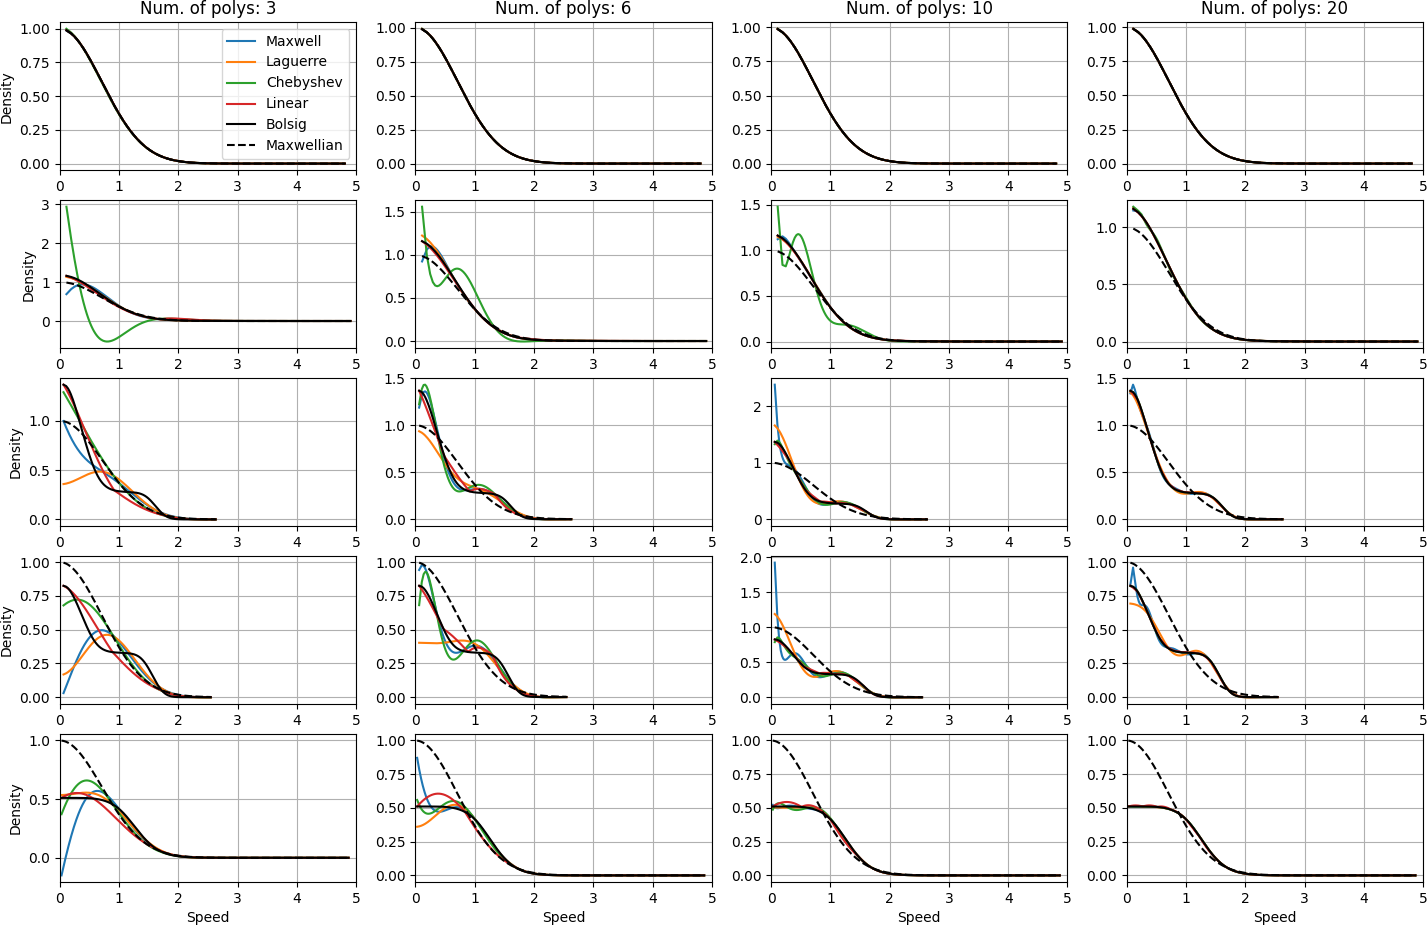
\includegraphics[height=2.in]{figures/bolsig_visual_lin.png}
\end{center}
%
\end{frame}

%===============================================================================
\begin{frame}
\frametitle{Investigation of different bases}
%
\begin{center}
   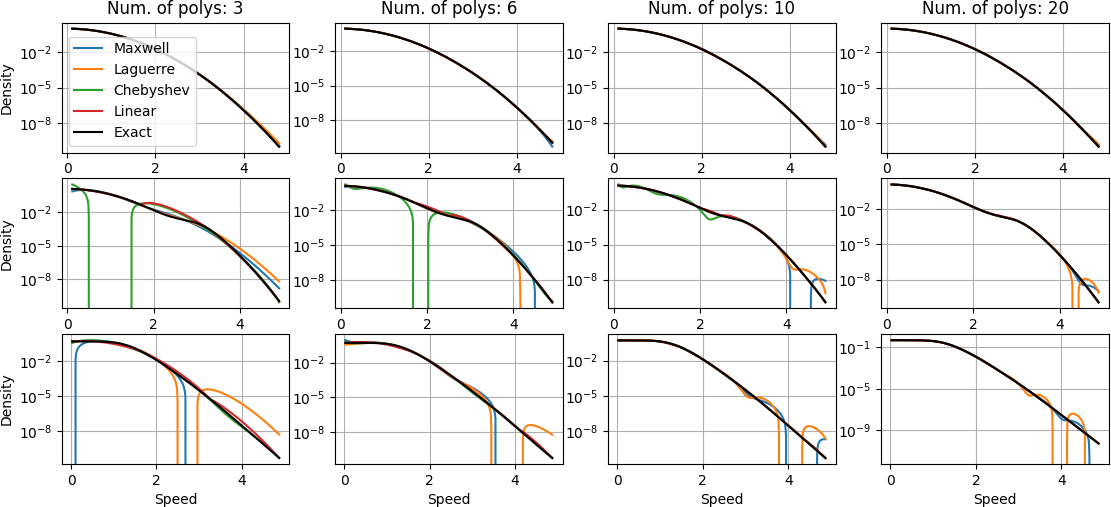
\includegraphics[height=2.in]{figures/bolsig_visual.png}
\end{center}
%
\end{frame}

%===============================================================================
\begin{frame}
\frametitle{Investigation of different bases}
%
\begin{center}
   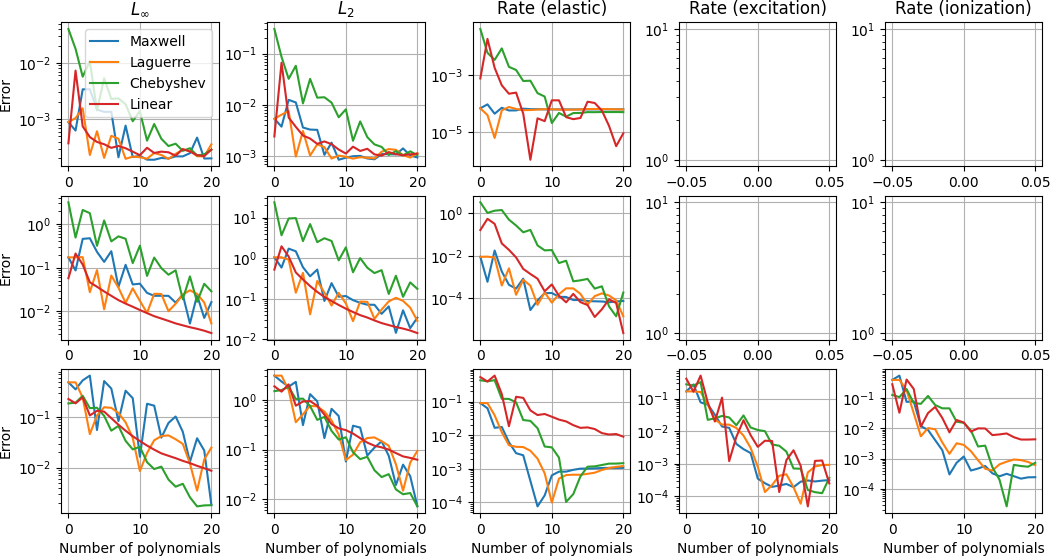
\includegraphics[height=2.in]{figures/bolsig_convergence.png}
\end{center}
%
\end{frame}


%===============================================================================

\begin{frame}
\frametitle{Implementation}
%
\begin{center}
   \includegraphics[height=2.in]{example-image-b}
\end{center}
%
\end{frame}


%===============================================================================
\end{document}
